\documentclass[11pt,preprint, authoryear]{elsarticle}

\usepackage{lmodern}
%%%% My spacing
\usepackage{setspace}
\setstretch{1.2}
\DeclareMathSizes{12}{14}{10}{10}

% Wrap around which gives all figures included the [H] command, or places it "here". This can be tedious to code in Rmarkdown.
\usepackage{float}
\let\origfigure\figure
\let\endorigfigure\endfigure
\renewenvironment{figure}[1][2] {
    \expandafter\origfigure\expandafter[H]
} {
    \endorigfigure
}

\let\origtable\table
\let\endorigtable\endtable
\renewenvironment{table}[1][2] {
    \expandafter\origtable\expandafter[H]
} {
    \endorigtable
}


\usepackage{ifxetex,ifluatex}
\usepackage{fixltx2e} % provides \textsubscript
\ifnum 0\ifxetex 1\fi\ifluatex 1\fi=0 % if pdftex
  \usepackage[T1]{fontenc}
  \usepackage[utf8]{inputenc}
\else % if luatex or xelatex
  \ifxetex
    \usepackage{mathspec}
    \usepackage{xltxtra,xunicode}
  \else
    \usepackage{fontspec}
  \fi
  \defaultfontfeatures{Mapping=tex-text,Scale=MatchLowercase}
  \newcommand{\euro}{€}
\fi

\usepackage{amssymb, amsmath, amsthm, amsfonts}

\def\bibsection{\section*{References}} %%% Make "References" appear before bibliography


\usepackage[round]{natbib}

\usepackage{longtable}
\usepackage[margin=2.3cm,bottom=2cm,top=2.5cm, includefoot]{geometry}
\usepackage{fancyhdr}
\usepackage[bottom, hang, flushmargin]{footmisc}
\usepackage{graphicx}
\numberwithin{equation}{section}
\numberwithin{figure}{section}
\numberwithin{table}{section}
\setlength{\parindent}{0cm}
\setlength{\parskip}{1.3ex plus 0.5ex minus 0.3ex}
\usepackage{textcomp}
\renewcommand{\headrulewidth}{0.2pt}
\renewcommand{\footrulewidth}{0.3pt}

\usepackage{array}
\newcolumntype{x}[1]{>{\centering\arraybackslash\hspace{0pt}}p{#1}}

%%%%  Remove the "preprint submitted to" part. Don't worry about this either, it just looks better without it:
\makeatletter
\def\ps@pprintTitle{%
  \let\@oddhead\@empty
  \let\@evenhead\@empty
  \let\@oddfoot\@empty
  \let\@evenfoot\@oddfoot
}
\makeatother

 \def\tightlist{} % This allows for subbullets!

\usepackage{hyperref}
\hypersetup{breaklinks=true,
            bookmarks=true,
            colorlinks=true,
            citecolor=blue,
            urlcolor=blue,
            linkcolor=blue,
            pdfborder={0 0 0}}


% The following packages allow huxtable to work:
\usepackage{siunitx}
\usepackage{multirow}
\usepackage{hhline}
\usepackage{calc}
\usepackage{tabularx}
\usepackage{booktabs}
\usepackage{caption}


\newenvironment{columns}[1][]{}{}

\newenvironment{column}[1]{\begin{minipage}{#1}\ignorespaces}{%
\end{minipage}
\ifhmode\unskip\fi
\aftergroup\useignorespacesandallpars}

\def\useignorespacesandallpars#1\ignorespaces\fi{%
#1\fi\ignorespacesandallpars}

\makeatletter
\def\ignorespacesandallpars{%
  \@ifnextchar\par
    {\expandafter\ignorespacesandallpars\@gobble}%
    {}%
}
\makeatother

\newlength{\cslhangindent}
\setlength{\cslhangindent}{1.5em}
\newenvironment{CSLReferences}%
  {\setlength{\parindent}{0pt}%
  \everypar{\setlength{\hangindent}{\cslhangindent}}\ignorespaces}%
  {\par}


\urlstyle{same}  % don't use monospace font for urls
\setlength{\parindent}{0pt}
\setlength{\parskip}{6pt plus 2pt minus 1pt}
\setlength{\emergencystretch}{3em}  % prevent overfull lines
\setcounter{secnumdepth}{5}

%%% Use protect on footnotes to avoid problems with footnotes in titles
\let\rmarkdownfootnote\footnote%
\def\footnote{\protect\rmarkdownfootnote}
\IfFileExists{upquote.sty}{\usepackage{upquote}}{}

%%% Include extra packages specified by user

%%% Hard setting column skips for reports - this ensures greater consistency and control over the length settings in the document.
%% page layout
%% paragraphs
\setlength{\baselineskip}{12pt plus 0pt minus 0pt}
\setlength{\parskip}{12pt plus 0pt minus 0pt}
\setlength{\parindent}{0pt plus 0pt minus 0pt}
%% floats
\setlength{\floatsep}{12pt plus 0 pt minus 0pt}
\setlength{\textfloatsep}{20pt plus 0pt minus 0pt}
\setlength{\intextsep}{14pt plus 0pt minus 0pt}
\setlength{\dbltextfloatsep}{20pt plus 0pt minus 0pt}
\setlength{\dblfloatsep}{14pt plus 0pt minus 0pt}
%% maths
\setlength{\abovedisplayskip}{12pt plus 0pt minus 0pt}
\setlength{\belowdisplayskip}{12pt plus 0pt minus 0pt}
%% lists
\setlength{\topsep}{10pt plus 0pt minus 0pt}
\setlength{\partopsep}{3pt plus 0pt minus 0pt}
\setlength{\itemsep}{5pt plus 0pt minus 0pt}
\setlength{\labelsep}{8mm plus 0mm minus 0mm}
\setlength{\parsep}{\the\parskip}
\setlength{\listparindent}{\the\parindent}
%% verbatim
\setlength{\fboxsep}{5pt plus 0pt minus 0pt}



\begin{document}



\begin{frontmatter}  %

\title{Question 2: Yield Spread}

% Set to FALSE if wanting to remove title (for submission)




\author[Add1]{Andrew Hyde}
\ead{23365935@sun.ac.za}





\address[Add1]{Stellenbosch University, South Africa}


\begin{abstract}
\small{
This analysis of the current yield spreads in the local bond market
places the current high spreads into historical context.
}
\end{abstract}

\vspace{1cm}





\vspace{0.5cm}

\end{frontmatter}



%________________________
% Header and Footers
%%%%%%%%%%%%%%%%%%%%%%%%%%%%%%%%%
\pagestyle{fancy}
\chead{}
\rhead{}
\lfoot{}
\rfoot{\footnotesize Page \thepage}
\lhead{}
%\rfoot{\footnotesize Page \thepage } % "e.g. Page 2"
\cfoot{}

%\setlength\headheight{30pt}
%%%%%%%%%%%%%%%%%%%%%%%%%%%%%%%%%
%________________________

\headsep 35pt % So that header does not go over title




\hypertarget{introduction}{%
\section{\texorpdfstring{Introduction
\label{Introduction}}{Introduction }}\label{introduction}}

Economists have recently pointed out that the current yield spreads in
local mid to longer dated bond yields have since 2020 been the highest
in decades.

\hypertarget{south-african-bond-yields}{%
\section{South African Bond Yields}\label{south-african-bond-yields}}

I begin by viewing the data and determine if there are any missing
values. I then plot the yields for bonds of differing maturities to
visualize the spread between the 3 Month, 2 year and 10 Year South
African bonds.

From the graph below, it does appear that the yield spreads in local mid
to longer dated bond yields have have increased since 2020 when compare
to historical spreads. The yield on the 3 year bond has decreased since
2015, this may be a reflection of anticipated interest rate cuts in the
near future. An increase in interest rates would imply an increase in
bond prices and thus yields would decrease.

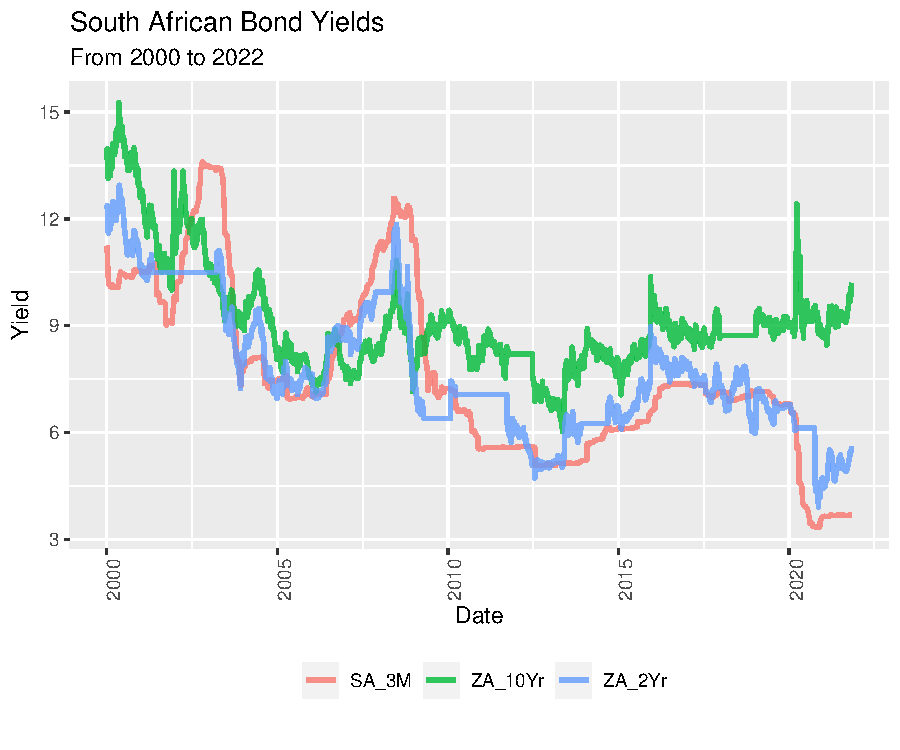
\includegraphics{Question2_files/figure-latex/unnamed-chunk-1-1.pdf}

To further investigate this topic I combine the available data for this
question using `left\_join'. I make use of this combined data set to
perform the rest analysis.

Using the combined data set, I plot out the the yields on mid and long
term South African Bonds from 2019 to 2022 to get an idea how the
spreads have changed since the pandemic.

The graph below illustrates how bond how mid and long term bond yields
have adjusted after the COVID-19 pandemic. It is not surprising that 2
year bond yields are down considerably since the pandemic first hit,
this may be the result of investors anticipating monetary easing through
lowered interest rates to combat the economic downturn of the pandemic.
This can be seen with sharp dive on the 2 year bond late in 2020. Since
then, the monetary authorities have been concerned with rising inflation
and so interest rate hikes have been taking place, which explains the
increases in the 2 year yields since late 2020.

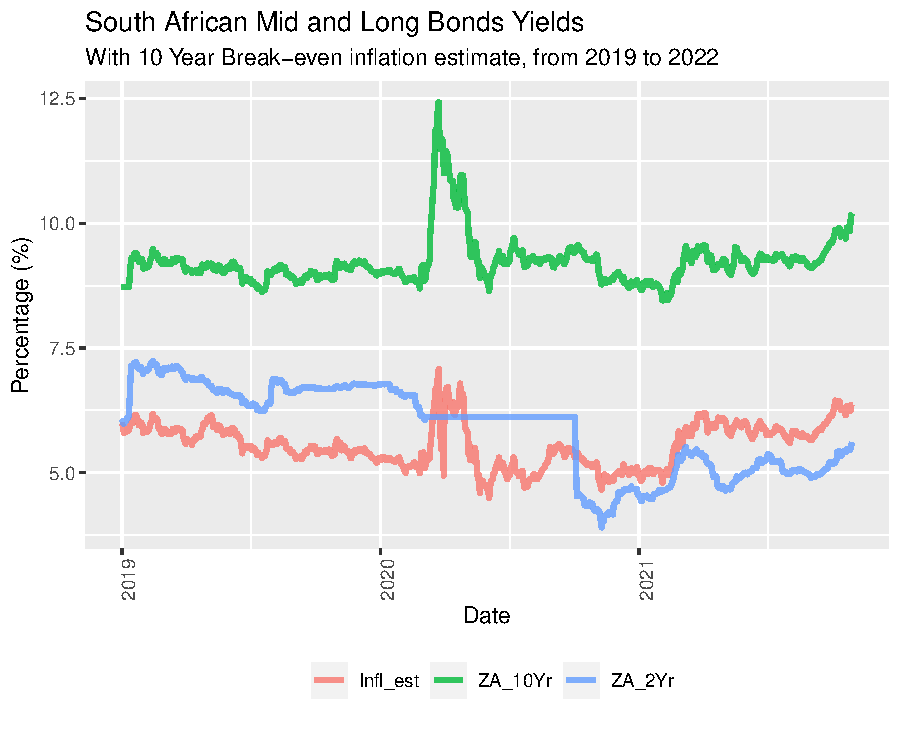
\includegraphics{Question2_files/figure-latex/unnamed-chunk-3-1.pdf}

\hypertarget{domestic-and-foreign-yields}{%
\section{Domestic and Foreign
Yields}\label{domestic-and-foreign-yields}}

I construct line graph and use `facet\_wrap' to display each variable on
its own axis. The graph shows the the mid to long term yield spread for
both South Africa and the United States over time, as well as the
prevailing interest rate at the time.

Over the past 5 years in both the local South African Bonds market and
the US Bonds Market, the mid to long term yield spread has widen for
both countries. However, as the RSA bond spread is larger it appears
that capital is flowing into South Africa to invest

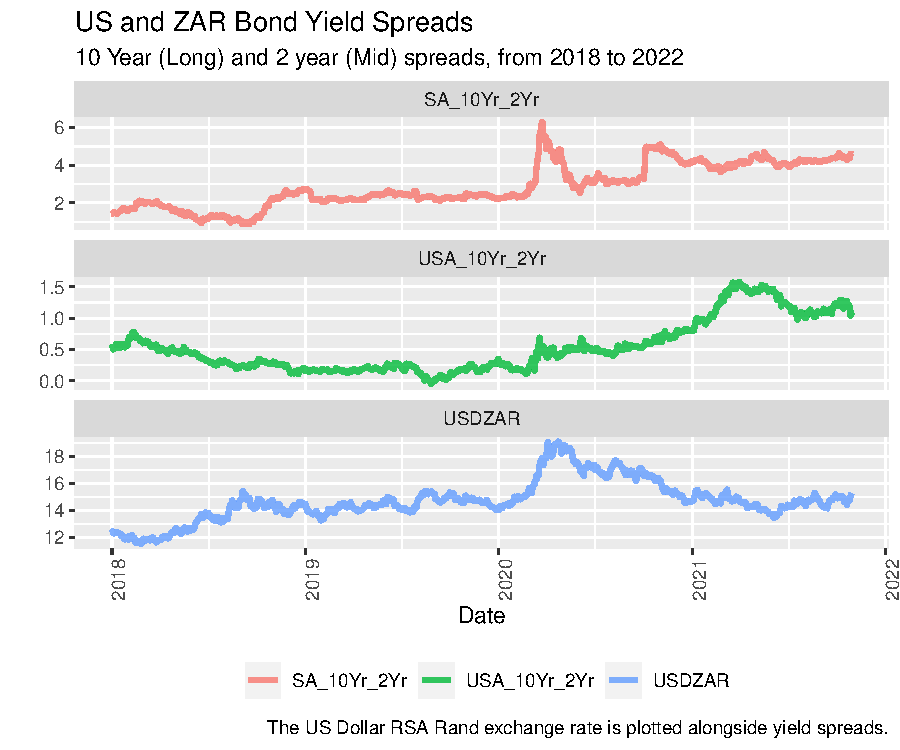
\includegraphics{Question2_files/figure-latex/unnamed-chunk-4-1.pdf}

I then plot the the 10 and 2 year yield spread of BRICS Countries along
with the VIX. I do this by calculating spreads for each country and then
select for these spread for the combined data set. The CBOE Volatility
Index has been added to the plot to provide of how yield spreads between
mid and long term bonds for the BRICS countries are increasing as
volatility expectations increase.

From the graph it appears that that there is a positive relationship
between volatility in the equities market implied by the VIX (when
looking at the VIX spike in early 2020) and the bond yield spreads.
Additionally, it appears that the yield spread between the more
developing BRICS countries (Brazil, India, South Africa) experiences a
widening of the yield spread since the beginning of the pandemic.

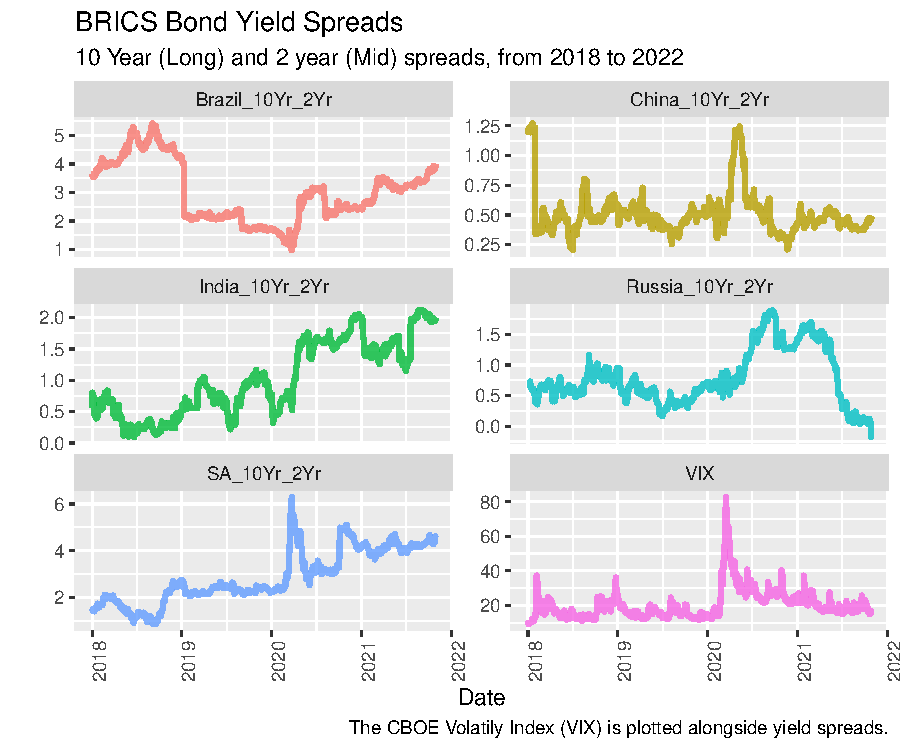
\includegraphics{Question2_files/figure-latex/unnamed-chunk-6-1.pdf}

\bibliography{Tex/ref}





\end{document}
